\documentclass[conference]{IEEEtran}
\usepackage{cite}
\usepackage{array}
\usepackage{graphicx}
\usepackage{amsthm}
\usepackage{amsmath}
\usepackage{amssymb}
\usepackage{mathrsfs}
% \usepackage{minted}
\usepackage{listings}
\usepackage{color} 						% red, green, blue, yellow, cyan, magenta, black, white

\usepackage{float} %used to force figures in a position
\hyphenation{op-tical net-works semi-conduc-tor}

\theoremstyle{definition}
\newtheorem{definition}{Definition}[section]

\begin{document}
\title{Clasificación de ECG usando Redes Neuronales}

\author{\IEEEauthorblockN{J. Agust\'{i}n Barrachina}
	\IEEEauthorblockA{Miembro Estudiantil IEEE\\
		Instituto Tecnol\'{o}gico de Buenos Aires\\}}
\maketitle

% \tableofcontents
% \newpage

\begin{abstract}
	Se clasificaron latidos de un segmento de señal de un electrocardiograma según el tipo de arritmia. El algoritmo utilizado fue un perceptrón multicapa usando backpropagation como clasificador. Se utilizaron PCA y SOM para reducir la dimensionalidad de los datos.
\end{abstract}

\section{Introducci\'{o}n}

El trabajo consistió en clasificar los latidos de un segmento de una señal de electrocardiograma de dos canales de 21 horas de duración según el tipo de arritmia.

El objetivo fue crear y entrenar un sistema que pueda reconocer y clasificar los distintos tipos de latidos.

\section{Data Set}

Se utilizaron las grabaciones de "MIT-BIH Long Term Database" \cite{MIT-BIH} disponible en el repositorio PhysioNet \cite{PHYSIONET}.

La grabación incluye anotaciones que identifican la posición y tipo de cada uno de los latidos presentes en la misma.

La grabación se identificará por el número 14172, y el identificador de la base de datos es "ltdb" (\underline{L}ong \underline{T}erm \underline{D}ata\underline{B}ase).
La misma presenta principalmente 4 tipos de latidos:

\begin{itemize}
	\item \textbf{Normales}. Identificados por la letra 'N'.
	\item \textbf{Ventriculares prematuros} Identificados por la letra 'V'.
	\item \textbf{Supraventriculares prematuros} Identificados por la letra 'S'.
	\item \textbf{Nodales prematuros} Identificados por la letra 'J'.
\end{itemize}

Para el tratamiento de los datos se utlizó la librería de python "wfdb" \cite{WFDB}.

\subsection{Reducción de Dimensionalidad}

Se usaron dos técnicas distintas para reducir la dimensión de los datos y así acelerar y facilitar las operaciones de la red neuronal.

La primera técnica fue la utilización de \textit{\underline{P}rincipal \underline{C}omponen \underline{A}nalysis} (PCA). La teoría del mismo no se desarrollará en éste informe.

Otra técnica utilizada fue la implementación de una red \textit{\underline{S}elf \underline{O}rganized \underline{M}ap} (SOM) que tampoco se desarrollará en este informe.

Finalmente se decidió optar por dejar la implementación del PCA por un motivo puramente de tiempo de ejecución, ya que la red SOM requería mucho tiempo de cómputo y no obtenía resultados perceptiblemente superiores a los de la red PCA. Se truncó las dimensiones de PCA reduciendo los datos de cada latido de 250 a 32.

\section{Diseño de la Red Neuronal}

Según Rezaul Begg et al. \cite{NN_HEALTHCARE}, la técnica más comúnmente utilizada de Redes Neuronales hasta el día de la fecha en procesamiento de ECG fue el perceptrón multicapa (MLP) entrenada con backpropagation (Sección 2 Capítulo 3), por dicho motivo se utilizará éste mismo como el algoritmo para utilizar en éste trabajo.

El mismo trabajo presenta una tabla (figura \ref{tab_tabla_comparacion_tecnicas}) que presenta diferentes aplicaciones de redes neuronales en el ámbito de cardiología. Lamentablemente ninguno de los casos es aplicable a nuestro caso ya que suelen ser diferenciación entre si y no sobre la probabilidad de tener AMI. Sin embargo, la mayoría de los casos usan una configuración de MLP de una sola capa oculta con lo cual en este trabajo se utilizará esa misma configuración.
Normalmente además se recomienda utilizar solo una capa ya que casi con seguridad no será necesario más capas.

\begin{figure}[H]
	\centering
	\includegraphics[width=8cm]{../out/ECG_table_techinques.png}
	\caption{Redes Neuronales Aplicadas en Cardiología según \cite{NN_HEALTHCARE}}
	\label{tab_tabla_comparacion_tecnicas}
\end{figure}

Si bien existen varios trabajos sobre la elección de la cantidad de elementos re la red oculta como \cite{SIZE1} o \cite{SIZE2}, no existe una receta única e infalible sobre cuántos nodos darle a la capa oculta. Para elegirlos se utilizaron las siguientes reglas \textit{RoT} (Rule of Thumb) que se describirán a continuación.

\begin{enumerate}
	\item \textit{Errar por más y no por menos:} Unos nodos extra no es probable que causen daño a la convergencia de la red, se los puede pensar como un exceso de capacidad. Mientras que usar pocos nodos pueden afectar a la convergencia. 
	\item \textit{Basado en la entrada y la salida:} Utilizar una cantidad de nodos que se encuentren entre la cantidad de nodos de la entrada y la cantidad de nodos de la salida. (Jeff Heaton autor de \textit{"Introduction to Neural Networks for Java"})
\end{enumerate}

Utilizando estas dos reglas se eligió utilizar la expresión \( nodos_{hidden} = (nodos_{entrada} + nodos_{salida})/1.5\).

Para el algoritmo de aprendizaje se utilizó una librería \cite{NIMBLENET} que implementa redes neurnales feed-forward (Redes Multicapa) permitiendo una variedad de algorimos de aprendizajes de backpropagation.

\subsection{Set de Entrenamiento}

En un primer momento se entrenaba la red con los primeros casos de latidos. Para dicho set de entrenamiento, el error aumentaba a medida que los datos estaban más alejados temporalmente de los mismos, es decir, si se tomaban los primeros 10 casos del set de datos para el entrenamiento, el conjunto de datos a partir del onceavo hasta el veinteavo mostraba grandes resultados, mientras que los datos rondando el número mil poseía resultados muy poco satisfactorios.

Para contrarrestar este problema se tomaron los datos de entrenamiento de forma aleatoria. Ésto logró mejorar mucho el desempeño pero a coste de tener mayor varianza en los resultados. Además el caso de seleccionar dos veces los mismos datos puede ocurrir con el código actual.

\section{Overfitting}

La implementación de la red presentó overfitting. Como se puede ver en los resultados listados a continuación, el error del set de datos del test set comienza a incrementar.

\begin{lstlisting}[frame=single]
Error: 	0.290525167175 	Epoch: 1000
Error: 	0.252432576731 	Epoch: 2000
Error: 	0.233333077085 	Epoch: 3000
Error: 	0.226507241997 	Epoch: 4000
Error: 	0.227502496085 	Epoch: 5000
Error: 	0.230580316278 	Epoch: 6000
Error: 	0.233771065888 	Epoch: 7000
Error: 	0.236764878811 	Epoch: 8000
Error: 	0.239612203297 	Epoch: 9000
Error: 	0.242385089641 	Epoch: 10000
\end{lstlisting}

La librería utilizada \cite{NIMBLENET} permite el uso de dropout para poder reducir el overfitting. El resultado a continuación muestra el caso para un dropout del 50\%.

\begin{lstlisting}[frame=single]
Error: 0.330238968525 	Epoch: 1000
Error: 0.254160001896 	Epoch: 2000
Error: 0.214160846981 	Epoch: 3000
Error: 0.193992225022 	Epoch: 4000
Error: 0.185100235993 	Epoch: 5000
Error: 0.180218777466 	Epoch: 6000
Error: 0.176489777988 	Epoch: 7000
Error: 0.173452841416 	Epoch: 8000
Error: 0.171893196978 	Epoch: 9000
Error: 0.172405423062 	Epoch: 10000
\end{lstlisting}

Se puede observar que el dropout mejoró notoriamente el overfitting haciendo que el mismo se de pasados las 9000 iteraciones.

\subsection{Cambio a la Librería}
Sin embargo el overfitting no se eliminó por completo y existe un número óptimo para el cual conviene no seguir entrenando la red. Por dicho motivo, se modificó la librería para poder realizar \textit{early stop}. 
La implementación permite elegir la cantidad de iteraciones con un aumento del error antes de abandonar el entrenamiento.  

\section{Implementación de la Red} \label{sec_config}

La siguiente figura (figura \ref{fig_diagram}, levemente modificada de la figura 6 de \cite{NN_HEALTHCARE}) muestra el diagrama básico de la implementación del proyecto.

\begin{figure}[H]
	\centering
	\includegraphics[width=8cm]{../out/diagrama.png}
	\caption{Diagrama general del proyecto}
	\label{fig_diagram}
\end{figure}

En primer lugar se extrae y se extraen varios vectores de dimensión 250 de cada caso de latido. 
Luego se reduce su dimensión utilizando PCA o SOM a una dimensión menor.
Finalmente se aplica la red multicapa obteniendo la salida \(y_i\) donde cada valor corresponde a una clasificación posible (\(0 \le y_i \le 1\) que representa la probabilidad de que el latido corresponda a dicha clasificación). 

\begin{itemize}
	\item Reducción de Dimensión usando PCA 32
	\item Configuración 32 - 20 - 4
	\item Función de activación: Sigmoidea 
	\item Cantidad de latidos de entrenamiento 10
	\item Dropout = 50%
	\item Early Stop de hasta 10 valores
\end{itemize}

\section{Análisis de los Resultados}

Para analizar los resultados se usaron dos parámetros que se los denominó \textit{aciertos} y los \textit{hallados}. 

El primero cuenta la cantidad de \textit{aciertos} de cada decisión, es decir, si se dijo que cierto numero de latidos corresponden a un categoría, cuántos de ellos realmente eran de esa categoría.

Por ejemplo, si encuentro 100 latidos 'N' y 90 de ellos lo eran, el porcentaje de aciertos será del 90\% lo cual parece ser un número muy aceptable. Sin embargo, si se alimentó la red con 900 latidos, solo el 10\% fueron hallados, haciendo que el desempeño de la red sea indeseado.

Por dicho motivo, para este segundo caso, se midió la cantidad de elementos de esa categoría encontrados o \textit{hallados} sobre el total real.

\section{Resultados}

La cantidad de aciertos totales fue superior al 70\% en la mayoría de los casos (recordar que como se usan sets se entrenamientos aleatorios en casa caso \ref{sec_config}, el mismo suele tener varianza).

Para una iteración con 2000 'N', 2000 'V', 1003 'S' y 148 'J', se tuvo un acierto de 77\% usando 10 casos de entrenamiento para cada categoría y un \textit{early stop} que termine el entrenamiento cuando la red aumenta 10 veces su error.

Los latidos que más satisfactoriamente se detectó fueron los Ventriculares ('V') en los cuales se obtuvo bajo varias condiciones, un resultado del 99\% tanto de \textit{aciertos} como de cantidad total \textit{hallada}.

Ésto último se le puede dar una explicación gráfica a partir de la red implementada SOM. El resultado de la misma se encuentra en la figura \ref{fig_som}. En dicha figura se puede ver claramente que los valores de los ventriculares están claramente definidos por lo cual es de esperar que se obtengan tan buenos resultados. Los normales y ventriculares poseen error pero en líneas generales tiene cierto grado de diferenciación. Los nodales prematuros por otro lado se superponen mucho con los demás resultados haciendo que en varios casos se interprete los demás casos (normales, ventriculares y supraventriculares) como un caso de nodales prematuros.

\begin{figure}[H]
	\centering
	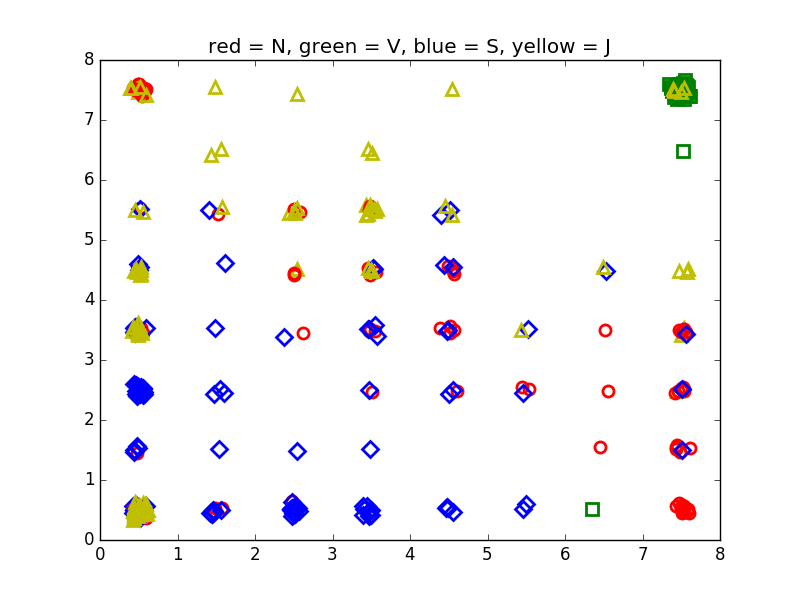
\includegraphics[width=9cm]{../out/CoolResults/som_weights.png}
	\caption{Resultados de una red SOM sobre algunos datos}
	\label{fig_som}
\end{figure}

Aproximadamente se obtuvo un \textit{porcentaje de enfermos ponderado} superior al 70\%.

\section{Posibles Mejoras}

Se podría implementar el método denominado como \textit{Cascade Correlation} (Fahlman et al. 1990) que permite ajustar dinámicamente la estructura de la red. La misma comienza con una red minimalista (perceptrón simple) y luego va ajustando los nodos de la capa oculta durante el entrenamiento.

Se debería seleccionar los datos de entrenamiento de una forma que asegure que los mismos no se repitan.

La librería permite definir funciones costo propias. Ésto se podría aprovechar para definir una función de costo propia que le otorgue menor peso a los casos Normales respecto a los demás.

La librería ofrece muchas variantes de backpropagation que no fueron probadas ni investigadas. Sería interesante inspeccionar sobre dichas variantes.

\IEEEpeerreviewmaketitle

\section*{Acknowledgment}

\newpage

\IEEEtriggeratref{8}
\bibliographystyle{IEEEtran}
\bibliography{ref}
\end{document}